%% LaTeX-Beamer template for KIT design
%% by Erik Burger, Christian Hammer
%% title picture by Klaus Krogmann
%%
%% version 2.1
%%
%% mostly compatible to KIT corporate design v2.0
%% http://intranet.kit.edu/gestaltungsrichtlinien.php
%%
%% Problems, bugs and comments to
%% burger@kit.edu

\documentclass[18pt]{beamer}
%% SLIDE FORMAT
\usepackage[utf8]{inputenc}
\usepackage{enumitem}
% use 'beamerthemekit' for standard 4:3 ratio
% for widescreen slides (16:9), use 'beamerthemekitwide'

%\usepackage{templates/beamerthemekit}
\usepackage{wrapfig}
\usepackage{hyperref}
\usepackage[noend]{algpseudocode}
\usepackage{graphicx}
\usepackage{epstopdf}

\epstopdfDeclareGraphicsRule{.gif}{png}{.png}{convert gif:#1 png:\OutputFile}
\AppendGraphicsExtensions{.gif}

 \newcommand{\R}{\mathbb{R}}
 \newcommand{\N}{\mathbb{N}}
 \newcommand{\Oh}{\mathcal{O}}
 \newcommand{\oh}{\mathrm{o}}
 \newcommand{\SP}{\mathrm{SP}}

% \usepackage{templates/beamerthemekitwide}

%\usepackage{epigraph}

% for quotes

\AtBeginSection[] % Do nothing for \section*
{
\begin{frame}<beamer>
\frametitle{Gliederung}
\tableofcontents[currentsection]
\end{frame}
}


\usepackage{biolinum}

\usepackage{pgfplots}

%% TikZ INTEGRATION

% use these packages for PCM symbols and UML classes
% \usepackage{templates/tikzkit}
% \usepackage{templates/tikzuml}

% the presentation starts here

\title[Algo I Tut]{10. Algorithmen Tutorium I}
\subtitle{Graphentheorie}
\author[Zangerle]{Konstantin Zangerle}

\institute{Institut für Theoretische Informatik}

\usepackage{listings}
\usepackage{color}

\definecolor{mygreen}{rgb}{0,0.6,0}
\definecolor{mygray}{rgb}{0.5,0.5,0.5}
\definecolor{mymauve}{rgb}{0.58,0,0.82}

\lstset{ %
  backgroundcolor=\color{white},   % choose the background color
  basicstyle=\footnotesize,        % size of fonts used for the code
  breaklines=true,                 % automatic line breaking only at whitespace
  captionpos=b,                    % sets the caption-position to bottom
  commentstyle=\color{mygreen},    % comment style
  escapeinside={\%*}{*)},          % if you want to add LaTeX within your code
  keywordstyle=\color{blue},       % keyword style
  stringstyle=\color{mymauve},     % string literal style
}

% Bibliography

\begin{document}
% change the following line to "ngerman" for German style date and logos
%\selectlanguage{ngerman}

%title page
\begin{frame}
\titlepage
\end{frame}

%table of contents
\begin{frame}{Gliederung}
 \tableofcontents
\end{frame}

\begin{frame}{Graphentheorie -- Grundbegriffe}
 \begin{itemize}
  \item Knoten
  \item Kante
  \item starke Zusammenhangskomponente
  \item Zusammenhängend
  \item Adjazenzmatrix
  \item Adjazenzarray
  \item Schleife
  \item ungerichtet
  \item gerichtet
  \item Breitensuche
  \item Tiefensuche
 \end{itemize}
\end{frame}

\begin{frame}{Graphentheorie -- Aufgabe}
\begin{columns}[onlytextwidth]
 \begin{column}{0.6\textwidth}
 \begin{itemize}
  \item geg. gerichteter, stark zusammenhängender Graphen
  \item existieren eind. Knotenid und Kantenids
  \item Knotenarray: für jeden Knoten einen Eintrag mit ID und einen Zeiger auf ein Array mit den ausgehenden Kanten
  \item Kantenarray: für jede Kante e einen Eintrag mit der Kanten-ID und ID des Zielknotens
 \end{itemize}
\end{column}
\begin{column}{0.4\textwidth}
 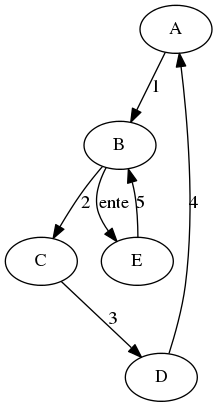
\includegraphics[scale=0.5]{beispielgraph.png}
\end{column}
\end{columns}
 
\end{frame}



\end{document}
